\addchap{Press F1 For Help}

\textit{Seminargruppen / Fachschaftsrat / Studierendenrat / Studienberatung / Studierendenwerk / Studiendekan / Studium mit Behinderung und chronischer Krankheit / Prüfungsamt}

Sollten irgendwann im Laufe deines Studiums Schwierigkeiten oder Fragen auftreten, scheue dich nicht rechtzeitig Hilfe in Anspruch zu nehmen.
Es gilt der Grundsatz: Lieber einmal zu oft gefragt, als einmal zu wenig, denn Fragen kostet bekanntlich ja nix. Und sind wir mal ehrlich, viele vor und nach dir werden vor ähnlichen Problemen gestanden haben und noch stehen.
Zum Glück gibt es zahlreiche Möglichkeiten Fragen zu klären, und Hilfe zu erhalten.
% G
Fachliche Fragen beantworten die jeweiligen Lehrenden und Tutoren immer gern. Zögere nicht lange und heb deinen Arm, du wirst sehen, dass viele deiner Kommilitoninnen und Kommilitonen dir dankbar sein werden. Denn auch wenn um dich herum alle bedächtig nicken, während vorne an der Tafel eine komplizierte Differenzialgleichung gelöst wird -- in Wahrheit haben die meisten genau wie du keine Ahnung.
Du bist am Anfang noch etwas schüchtern? Dann merke dir deine Frage und gehe vor oder nach der Veranstaltung nach vorne.

Mit der Zeit lernst du sicherlich auch Kommilitonen älterer Semester kennen, die du um Hilfe bitten kannst. 
Das gilt dann aber nicht nur für inhaltliche Fragen zu einer Vorlesung, sondern auch zum Studienablauf.
Wie funktioniert das mit der Anrechnung dieses Moduls? Wann kann ich mich für Prüfungen einschreiben? Wo muss ich mich melden, wenn ich bei einer Prüfung krank war? Im Zweifelsfall kontaktierst du den Fachschaftsrat. Dort ist Vertrautheit auch keine Frage und du bekommst meistens schnell eine Antwort auf deine Frage genannt oder zumindest die Ansprechperson, die dir diese geben kann.

\refstepcounter{dummy}\label{sec:seminargruppen}
\minisec{Seminargruppen}
Damit du dich am Anfang des Studiums schnell zurechtfindest, wirst du für das erste Semester gemeinsam mit anderen Studierenden in eine Seminargruppe eingeteilt.
Ihr teilt euch einen gemeinsamen Stundenplan.
In den Übungen wirst du damit immer wieder vertraute Gesichter sehen, mit denen du dich zu Lerngruppen zusammentun kannst.
Ganz oft entstehen dabei neue Freundschaften.
% G
Als direkte Ansprechperson für Fragen oder Probleme steht dir jederzeit dein Seminargruppenmentor zur Verfügung.
Im Verlauf des ersten Semesters gibt es mehrere Treffen, bei denen wichtige Informationen zu Ablauf und Organisation des Studiums vermittelt werden. Die Termine solltest du daher auf keinen Fall verpassen.

%\newpage

\refstepcounter{dummy}\label{sec:fachschaftsrat}
\minisec{Fachschaftsrat (FSR)}
\begin{wrapfigure}{r}{3cm}\ \\[-1cm]
\flushright
\includegraphics[width=\linewidth, trim=160 150 150 50, clip]{img/fsr_logo}
\end{wrapfigure}

Der Fachschaftsrat ist deine studentische Vertretung auf Fakultätsebene.
Er wird jährlich gewählt und besteht derzeit aus 17 Mitgliedern der Fachschaft Informatik. Zu dieser gehören alle Studierenden der Fakultät.
 
\textbf{Aufgaben} \\
Für dich ist der FSR die erste Anlaufstelle bei Problemen oder Fragen zu deinem Studium. Er bietet viele nützliche Tipps und Hilfestellungen wie Klausurensammlungen \link{ftp://ftp.ifsr.de/klausuren} und Beratungsangebote, von denen du jederzeit gern Gebrauch machen kannst. Zusätzlich zur Unterstützung im Studium versucht der FSR auch dein Leben jenseits der Uni durch soziale, kulturelle Angebote ein bisschen angenehmer zu machen.

So veranstaltet er meistens einmal pro Monat, Spieleabende mit Brett-, Karten- und digitalen Spielen in der Fakultät. Traditionell findet auch schon während der Erstsemestereinführung ein solcher statt. 
Er ist Mitorganisator von Weihnachtsfeiern, Grillabenden, Wanderungen, Sportturnieren und vielem mehr.
% G
Nicht zuletzt organisiert er zusammen mit vielen Helferinnen und Helfern eine Woche lang die Erstsemestereinführung und hat für dich dieses Heft erstellt.

Der FSR ist auch zentraler Bestandteil der studentischen Mitwirkung in Hochschulgremien, Ausschüssen und Kommissionen. 
Dort hat er dann beispielsweise direkten Einfluss auf die Überarbeitung von Studienordnungen und die Berufung von Professorinnen und Professoren an deiner Fakultät. 
Er hilft bei der Qualitätskontrolle und -verbesserung der Lehre mit, indem er zum Beispiel Evaluationen von Vorlesungen durchführt.

\begin{figure}[h!]
\centering
\includegraphics[width=\textwidth]{img/fsr_gewaehlt_assoziiert_1617}
\caption*{\small \textit{Gewählte Mitglieder und Assoziierte deines FSR in der Legislatur 2016/2017.}}
\end{figure}

\textbf{Verleih} \\
Der FSR bietet für alle Studierenden der TU Dresden verschiedene Geräte und Materialien zum Ausleihen an \link{https://www.ifsr.de/service:leihen}. 
Ausgeliehen werden können unter anderem verschiedene Raspberry Pi, eine Oculus Rift und Lego Mindstorms Roboter.
Schau einfach vorbei und bring beim ersten Mal deinen Personalausweis mit, damit dir gleich ein Leihschein ausgestellt werden kann. 
Es gibt keine Ausleihgebühren, allerdings kann unter Umständen eine Kaution fällig sein.

\textbf{Kontakt} \\
Das Büro des FSR befindet sich im Erdgeschoss des Fakultätsgebäudes (APB/E017). Während der Vorlesungszeit ist dieses meistens durchgehend besetzt. Besucherinnen und Besucher sind immer willkommen. Neuigkeiten werden meistens über die sozialen Kanäle wie Facebook \link{https://www.facebook.com/iFSR.de/} und Twitter \link{https://twitter.com/ifsr} verbreitet. Natürlich kannst du über diese Plattformen auch Kontakt aufnehmen oder einfach eine E-Mail an \textit{fsr@ifsr.de} schreiben.

\textbf{Der FSR braucht dich} \\
Die Universität wird in vielen Bereichen demokratisch von unten nach oben gesteuert. Diese Demokratie lebt vom Mitmachen und von Menschen, die Ideen, Projekte und Visionen umsetzen.
Das funktioniert seit vielen Jahrzehnten erfolgreich.
Damit das so bleibt, braucht der FSR, genau wie viele andere Organe und Gruppen an der Universität jederzeit aktive, engagierte, motivierte Mitglieder und Unterstützende.

Auch wer sich nicht selbst zur Wahl aufstellen lassen will, kann etwas für seine Fachschaft tun.
Der erste Schritt ist wählen zu gehen, das kostet nun wirklich kaum Zeit und ist wichtig, um den FSR zu legitimieren und ihm Rückhalt für die Vertretung der studentischen Interessen zu geben.
Und wie wäre es zum Beispiel, wenn du im nächsten Jahr selbst bei der ESE mitwirkst? Oder vielleicht einen Programmierkurs leitest?
Es sind zum Beispiel auch immer Organisationstalente und Mitwirkende für einzelne Veranstaltungen wie die Sportturniere oder die Lange Nacht der Wissenschaften gesucht.

Wenn du dich also nicht das ganze Jahr lang offiziell gewählt engagieren willst, kannst du jederzeit mithelfen und -wirken, Aufgaben oder Ideen gibt es genug und du darfst gerne deine eigenen mitbringen. 

\begin{figure}[h!]
\centering
\textit{Studierendenvertretung ist, was du draus machst.}
\end{figure}

Jeden Montag trifft sich der FSR um 18:45 Uhr im großen Ratssaal (APB/1004), um unter anderem über verschiedenste Themen, wie beispielsweise die Gremienarbeit, anstehende Veranstaltungen und Demos, aber auch über Probleme und Entwicklungen an der Fakultät und Universität zu diskutieren.
Du bist herzlich eingeladen und kannst einfach vorbeikommen, denn die Sitzungen sind in der Regel für alle öffentlich. Auf der Webseite des FSR \link{https://www.ifsr.de} findest du neben den Sitzungsprotokollen \link{https://www.ifsr.de/fsr:sitzung} viele weitere nützliche Informationen.

\minisec{Studierendenrat (StuRa)}
Der Studierendenrat, in anderen Bundesländern oftmals als Allgemeiner Studierendenausschuss (AStA) und Studierendenparlament (StuPa) bekannt, ist das den Fachschaftsräten übergeordnete Organ und vertritt die Interessen aller Studierenden der TU Dresden. Er bietet eine Reihe von Serviceleistungen an, dazu gehören:
\begin{itemize}
\item BAföG- und Sozialberatung
\item Rechtsberatung
\item Beratung für ausländische Studierende
\item Beratung für Studierende mit Kind
\item Beratung zu Anträgen und Förderungsmöglichkeiten
\item Verkauf von Karten für verschiedene Kulturveranstaltungen
%\item Material- und Geräteverleih (mittlerweile nicht mehr, oder?)
\end{itemize}

Detaillierte Informationen und vieles mehr finden sich auf der Webseite des StuRa \link{https://www.stura.tu-dresden.de}.

% Wird der gedruckte Spirex eigentlich noch aktualisiert? Die PDF ist von 2014/15 :/

\newpage
\mbox{}
\thispagestyle{empty}
\AddToShipoutPicture*{\put(0,0){%
\parbox[b][\paperheight]{\paperwidth}{%
\centering
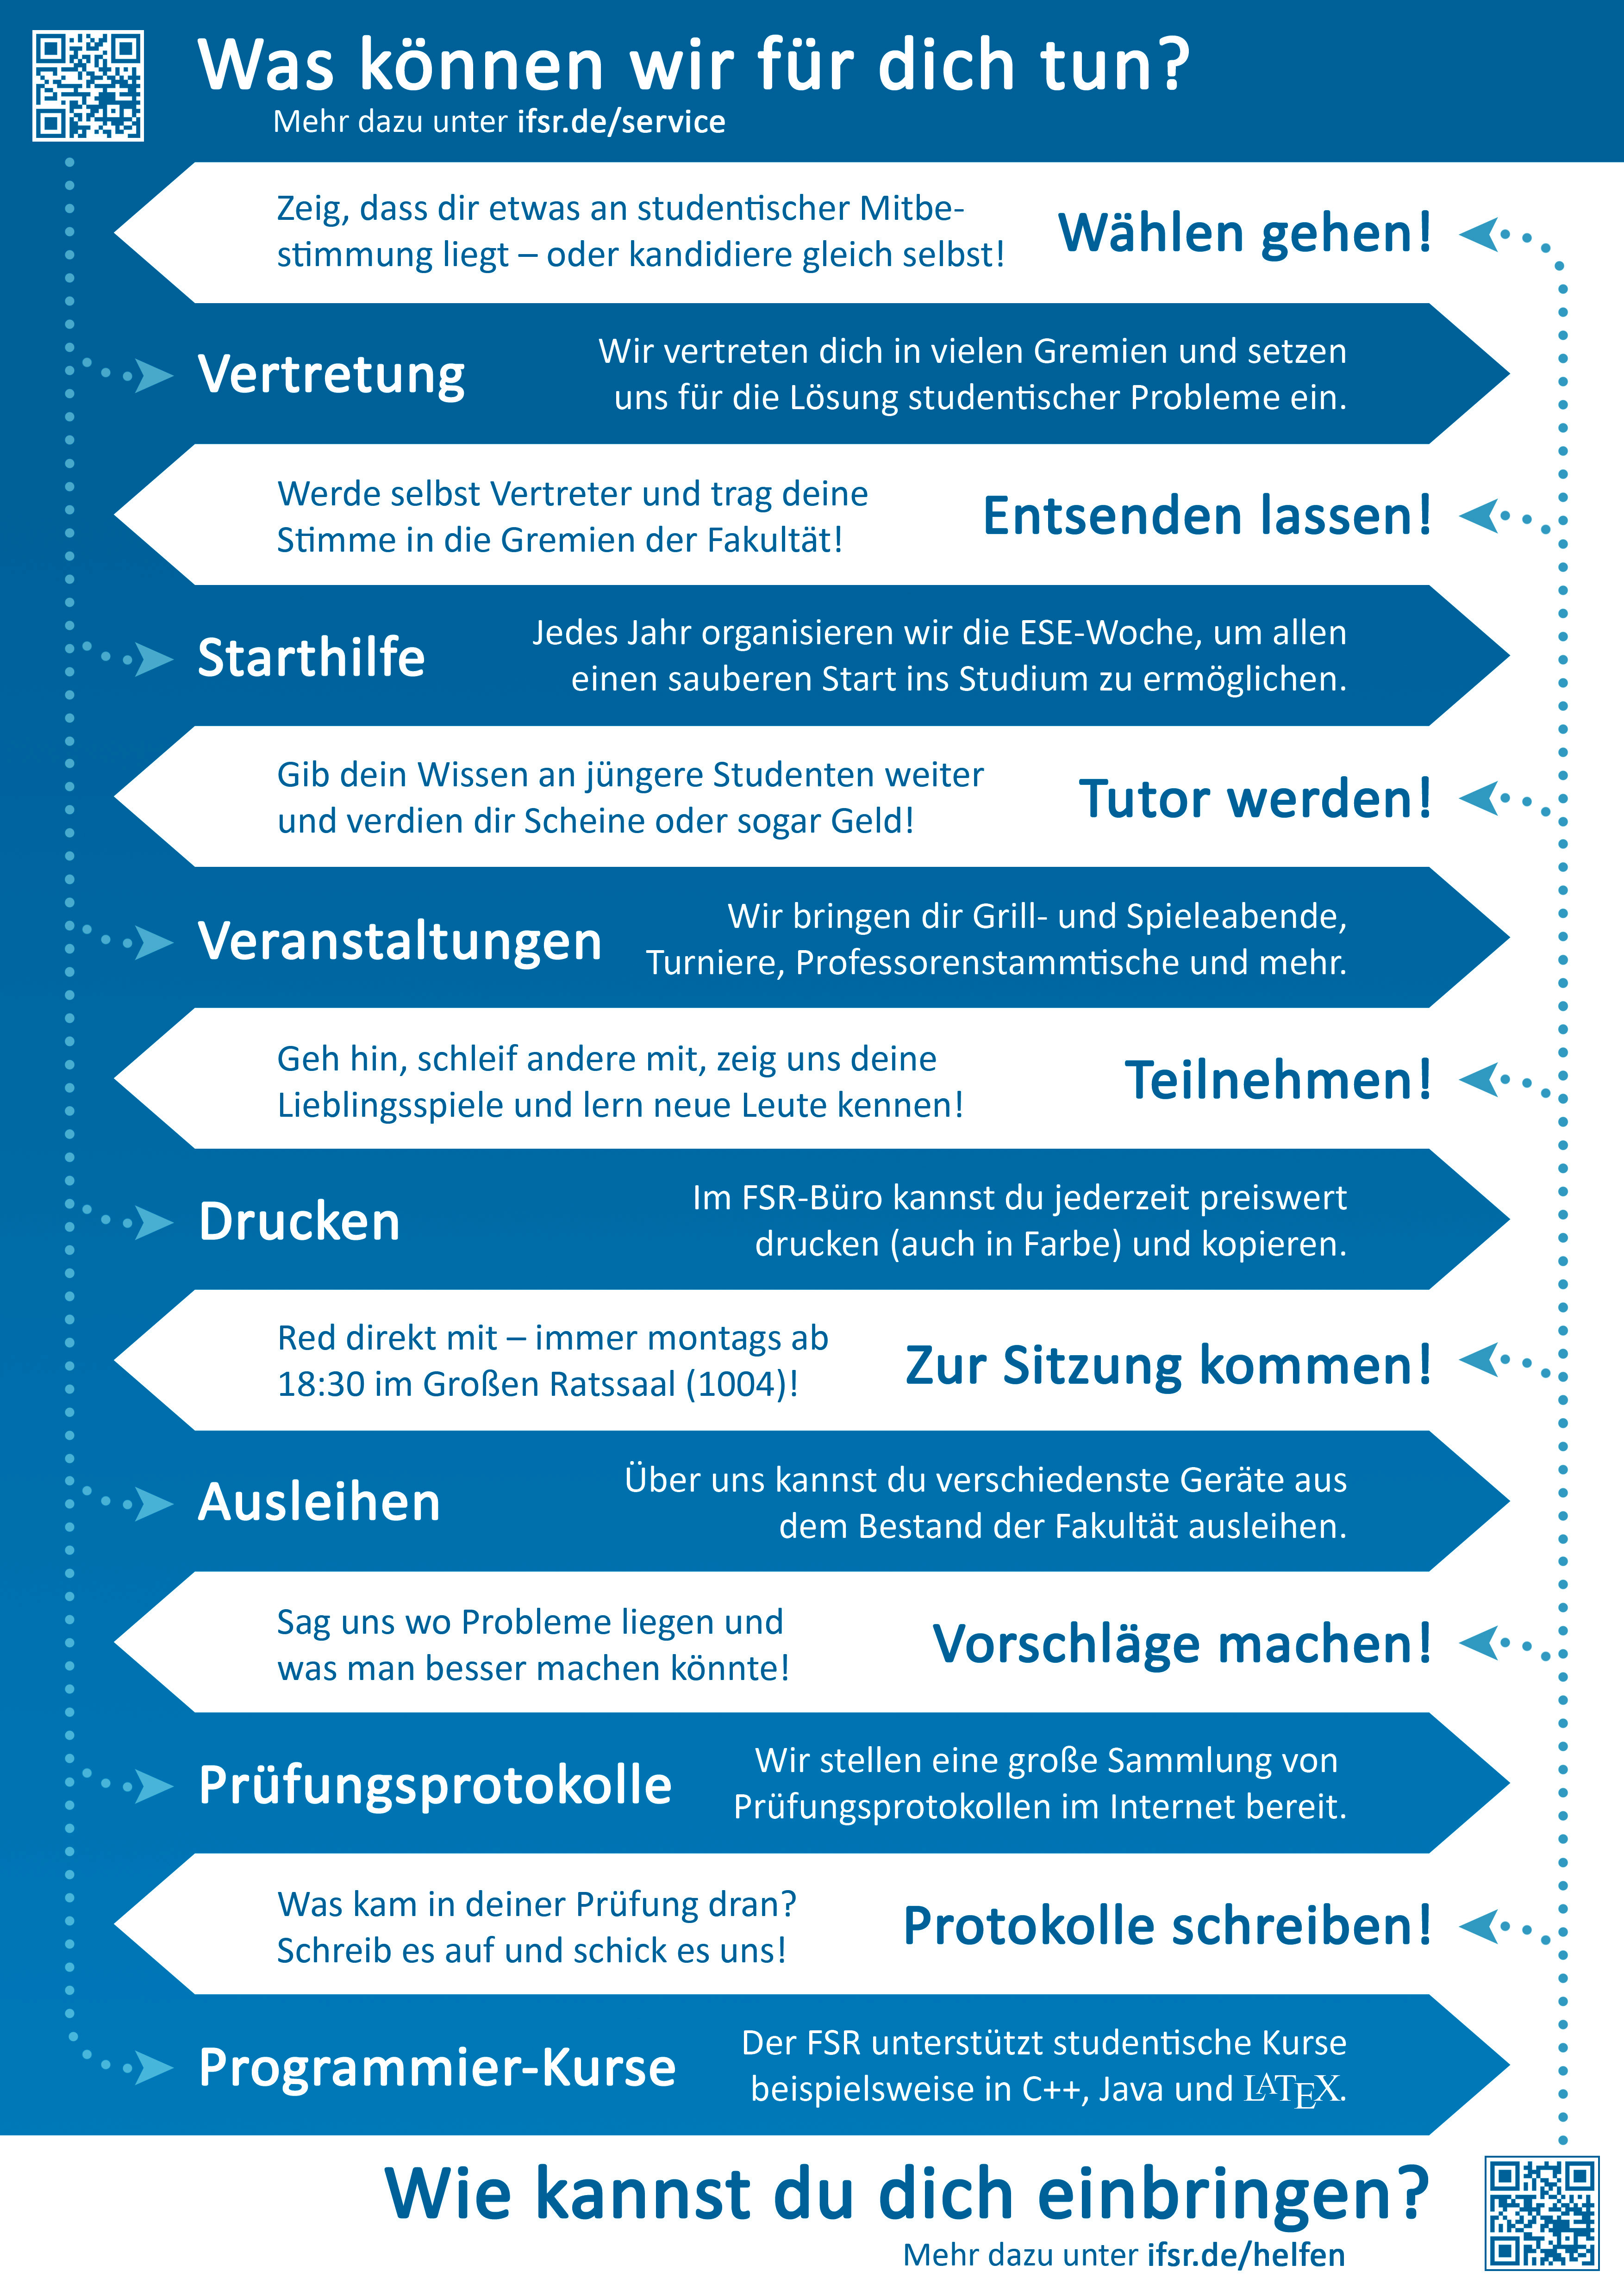
\includegraphics[width=\dimen107,height=\dimen108,keepaspectratio]{img/fsr_und_du-tinted.jpg}%
\vfill
}}}

\newpage

\minisec{Studienberatung}
Manchmal verläuft das Studium nicht reibungslos.
Einzelne Studierende haben gerade zu Beginn des Studiums Orientierungsschwierigkeiten oder Probleme bei der Bewältigung der Anforderungen.
Die Studienberatung unterstützt dich mit Informationsangeboten in allen Phasen deines Studiums.
Die Beratung erstreckt sich beispielsweise auf Fragen zu Prüfungen und Prüfungsvorbereitung, Spezialisierungsmöglichkeiten, Studienfachwechsel oder Fragen zur Stundenplangestaltung.

Die TU Dresden bietet eine allgemeine, fakultätsübergreifende Studienberatung an \link{https://tu-dresden.de/studium/im-studium/beratung-und-service/zentrale-studienberatung}. Diese kann zum Beispiel bei Zweifeln an der Studiengangswahl, Prüfungsangst oder ähnlichem Hilfe leisten. Für alle studiengangsspezifischen Fragen und Probleme gibt es an unserer Fakultät jeweils eigene Beratungsangebote mit Ansprechpersonen auf studentischer und nicht-studentischer Seite \link{https://tu-dresden.de/ing/informatik/studium/beratung}.

\minisec{Studierendenwerk (StuWe)}
Das Studierendenwerk betreibt nicht nur die Wohnheime und sorgt für gute und günstige Verpflegung in Mensen und Cafeterien, sondern bietet eine umfangreiche Betreuung und Förderung für Studierende an. Dazu zählen:

\begin{itemize}
\item Rechts- und Sozialberatung
\item Psychosoziale Beratung
\item Bearbeitung von BAföG-Anträgen
\item Bearbeitung von Anträgen auf Umzugsbeihilfe
\item Hilfestellung für Studierende mit Handicaps
\item Schwangerschaft und Kinderbetreuung im Studium
\end{itemize}

Weitere Informationen zu den Aufgaben und Angeboten des StuWe findest du im Internet \link{https://www.studentenwerk-dresden.de/}.

\minisec{Studiendekan und Studienbeauftragter}
In der Fakultät gibt es viele verschiedene Ämter. 
Das höchste und wichtigste ist die Rolles des Dekans der Fakultät und seinem Stellvertreter, dem Prodekan. 
Für die Lehre und damit dein Studium ist allerdings der sogenannte Studiendekan von großer Bedeutung.
Er ist für die Angelegenheiten der Lehre in der Fakultät zuständig, vermittelt zwischen Studierenden und Lehrenden und hilft bei Problemen mit dem Studium allgemein.

\textbf{Studiendekan für deutschsprachige Studiengänge}\\
Prof. Dr. rer. nat. habil. Weber \\
Büro: APB/1055 \\
Telefon: (0351) 463-38477 \\
E-Mail: gerhard.weber@tu-dresden.de

\textbf{Studiendekan für englischsprachige Studiengänge}\\
Prof. Dr. Christof Fetzer \\
Büro: APB/3104 \\
Telefon: (0351) 463-39709 \\
E-Mail: christof.fetzer@​tu-dresden.de

\textbf{Studienbeauftragter für Lehramtsstudiengänge}\\
Dr. Sven Hofmann \\
Büro: APB/2096 \\
Telefon: (0351) 463-38306 \\
E-Mail: sven.hofmann@​tu-dresden.de

\minisec{Studium mit Behinderung und chronischer Krankheit}

An der TU Dresden wird stets an einer barrierearmen Gestaltung des Studiums sowie der Studienumgebung gearbeitet.
Wenn du gesundheitlich beeinträchtigt bist, ergeben sich oftmals besondere Fragen und Themen rund ums Studium. 
Für eine chancengerechte Teilnahme am Studium stehen dir zahlreiche Unterstützungs- und Beratungsangebote zur Verfügung \link{https://tu-dresden.de/studium/rund-ums-studium/studieren-mit-beeintraechtigung}.


\refstepcounter{dummy}\label{sec:pruefungsamt}
\minisec{Prüfungsamt (PA)}
Das Prüfungsamt ist für die Prüfungseinschreibung, Bekanntgabe der Ergebnisse und viele weitere Dinge rund ums Thema Prüfungen zuständig. 
Du findest viele Informationen, Anträge und häufig gestellte Fragen im Netz \link{https://tu-dresden.de/ing/informatik/studium/pruefungsorganisation}. 
Während der Sprechzeiten kannst du auch ohne vereinbarten Termin im Raum APB/3039 deine Anträge und Fragen loswerden oder unter \textit{(0351) 463-38230} anrufen.

\textbf{Sprechzeiten in der}

\begin{multicols}{2}
\textbf{Vorlesungszeit} \\
Di, Do: 12.30 - 15.00 Uhr\\
Mi: 09.00 - 11.00 Uhr\\
Mo, Fr: geschlossen	

\textbf{Vorlesungsfreie Zeit} \\
Di, Do: 12.30 - 15.00 Uhr\\
Mo, Mi, Fr: geschlossen
\end{multicols}
